% !TEX program = xelatex
% !BIB program = bibtex
\documentclass[11pt, openright, twoside]{report}
\usepackage[english,portuguese]{babel}

\selectlanguage{english}

%% %%%%%%%%%%%%%%%%%%%%%%%%%%%%%%%%%%%%%%%%%%%%%%%%%%%%%%%%%%%%%%%%%%%%%%%%%%%%
%% %%%%%%%%%%%%%%%%%%%% IMPORTANT: SET THE INFORMATION %%%%%%%%%%%%%%%%%%%%%%%%
%% %%%%%%%%%%%%%%%%%%%%%%%%%%%%%%%%%%%%%%%%%%%%%%%%%%%%%%%%%%%%%%%%%%%%%%%%%%%%
\newcommand{\departmentname}{INFORMÁTICA}
\newcommand{\thesisname}{Formalization and Runtime Verification of Invariants for Robotic Systems}
\newcommand{\studentname}{Ricardo Jorge Dias Cordeiro}
\newcommand{\coursename}{Engenharia Informática}
\newcommand{\specname}{Especialização em Interação e Conhecimento}
\newcommand{\versaoprovisoria}{Versão Provisória} % TODO: Blank for final version
\newcommand{\thesistype}{Dissertação}
\newcommand{\alcides}{Alcides Miguel Cachulo Aguiar Fonseca}
%\newcommand{\thirdadvisor}{Se aplicável, nome completo do terceiro orientador}
%% %%%%%%%%%%%%%%%%%%%%%%%%%%%%%%%%%%%%%%%%%%%%%%%%%%%%%%%%%%%%%%%%%%%%%%%%%%%

% -----------------------------------------------------------------------------
% Packages defined by the student
%% %%%%%%%%%%%%%%%%%%%%%%%%%%%%%%%%%%%%%%%%%%%%%%%%%%%%%%%%%%%%%%%%%%%%%%%%%%%
%% Important packages
\usepackage{times}
\usepackage{graphicx}
\usepackage{subcaption}

\usepackage{csquotes}
\usepackage{makeidx}

% Packages for the cover
\usepackage{fontspec}
\newfontfamily{\coverfont}{arial-narrow}
    [Path = ./assets/, 
    Extension = .ttf, 
    UprightFont = *-regular,
    BoldFont = *-bold
    ]
\usepackage{anyfontsize}
\usepackage{afterpage}

\usepackage{changepage}

% Positioning
\usepackage{float}

% Page format
\usepackage[dvips]{geometry}
\geometry{
    a4paper=true,
    portrait=true,
    left=2.5cm,
    right=2.5cm,
    top=2.5cm,
    bottom=2.5cm
}

%% %%%%%%%%%%%%%%%%%%%%%%%%%%%%%%%%%%%%%%%%%%%%%%%%%%%%%%%%%%%%%%%%%%%%%%%%%%%%
%% Other required packages

% Bibliography
\bibliographystyle{plainnat}
\usepackage[numbers]{natbib}

% Math
\usepackage{amsmath}
\usepackage{amssymb} 
\usepackage{amsthm}

% Images
\usepackage{color}
\usepackage[table, xcdraw,dvipsnames]{xcolor}

% Code listings
\usepackage{caption} 
\usepackage{listings}

% Text and pdf
\usepackage{pdfpages}
\usepackage{xspace}
\usepackage[shortlabels]{enumitem}

% Links
\usepackage[colorlinks=true, citecolor=Blue]{hyperref}
\usepackage[all]{hypcap}
\usepackage{cleveref}

%BNF grammars
%\usepackage{simplebnf}


% Generated the pdf with information
\hypersetup{
    pdfauthor={\studentname},                                       
    pdftitle={\thesisname},                                         
    pdfsubject={\thesistype in \coursename},                        
    pdfkeywords={Keyword1, Keyword2, Keyword3, Keyword4}                 % TODO
}

%% %%%%%%%%%%%%%%%%%%%%%%%%%%%%%%%%%%%%%%%%%%%%%%%%%%%%%%%%%%%%%%%%%%%%%%%%%%%%
%% Other packages




%% %%%%%%%%%%%%%%%%%%%%%%%%%%%%%%%%%%%%%%%%%%%%%%%%%%%%%%%%%%%%%%%%%%%%%%%%%%%%
%% Auxiliary commands
\newcommand{\cleanpage}{\newpage\mbox{}\thispagestyle{empty}\newpage}

\newcommand{\startpagecounter}[1]{\setcounter{page}{1}\pagenumbering{#1}}

% Commands for TODOS
\newcommand{\nb}[2]{\fcolorbox{gray}{yellow}{\bfseries\sffamily\scriptsize#1}{\sf\small$\blacktriangleright$\textit{#2}$\blacktriangleleft$}}
\newcommand\todo[1]{\nb{Todo}{#1}}

\newcommand{\missref}{\fcolorbox{gray}{red}{\bfseries\sffamily\scriptsize\textcolor{white}{REF}}}


% -----------------------------------------------------------------------------

% Index
\makeindex

% -----------------------------------------------------------------------------
% Begin of the thesis
\begin{document}

\startpagecounter{roman}

% Cover
% !TeX root = ../main.tex
% %%%%%%%%%%%%%%%%%%%%%%%%%%%%%%%%%%%%%%%%%%%%%%%%%%%%%%%%%%%%%%%%%%%%%%%%%%%%%
% %%%%%%%%%%%%%%%%%%% Cover: No need to change anything here %%%%%%%%%%%%%%%%%% 
% %%%%%%%%%%%%%%%%%%%%%%%%%%%%%%%%%%%%%%%%%%%%%%%%%%%%%%%%%%%%%%%%%%%%%%%%%%%%%
\thispagestyle{empty}

% Sets the new page geometry
\newgeometry{
    left=3cm,
    right=3cm,
    top=1cm,
    bottom=0.4cm
}

% Set the cover font to Arial Narrow
{\coverfont

% Center the page text
\begin{center}

% Universidade de Lisboa, Faculdade de Ciências, Departamento de Informática
{\large 
UNIVERSIDADE DE LISBOA
\vspace{8.0pt}

FACULDADE DE CIÊNCIAS
\vspace{8.0pt}

DEPARTAMENTO DE \departmentname
\vspace{8.0pt}
}

\vspace{46pt}

% Ciências ULisboa Logo

\includegraphics{images/logotipo.png}

\vspace{117pt}

% Title of the thesis
{\fontsize{17}{19.55}\coverfont\textbf{\thesisname}}

\vspace{110pt}

% The student name
{\fontsize{15}{17.25}\coverfont\studentname}

\vspace{74pt}

% Designação do curso e especialidade
{\fontsize{13}{14.95}\coverfont\textbf{Mestrado em {\coursename}}

\vspace{0.65pt}

\specname
}

\vspace{22pt}

% Versão Provisória
{\fontsize{11}{12.65}\coverfont\versaoprovisoria}

\vspace{27pt}

% Supervisors
{\fontsize{13}{14.95}\coverfont
{\thesistype} orientad\ifthenelse{\equal{\thesistype}{Dissertação}}{a}{o} por: 

\firstadvisor

\vspace{3pt}

\secondadvisor

\vspace{3pt}

\thirdadvisor
}

~
\vfill

% Year the work was done
{\Large\the\year{}}

\end{center}
}

% Restore the page geometry
\restoregeometry
\cleanpage

% Acknowledgements
% !TeX root = ../main.tex
% %%%%%%%%%%%%%%%%%%%%%%%%%%%%%%%%%%%%%%%%%%%%%%%%%%%%%%%%%%%%%%%%%%%%%%%%%%%%%%
% Acknowledgements
\selectlanguage{english}

\pagestyle{plain}

\vspace*{2cm}
\begin{center}
\Large \bf Acknowledgments
\end{center}
\vspace*{1cm} \setlength{\baselineskip}{0.6cm}

I would like to thank my coordinator, Prof. Alcides Fonseca, for the exceptional way of teaching not only through the making of my thesis but also throughout all my academic courses. 

My coordinator Prof. Chris Timperley for taking his time to help me in this chapter of his life where he had to take care of his baby. 

My upperclassman Paulo and Catarina, for all the advice and help. 

All my friends who spent time with me know that somehow you helped me through this process. 

All my family, in particular my grandparents. 

My little brother. 

In the end, and more importantly, my mother for taking care of me all my life and giving me the opportunity to follow this path.

\cleardoublepage~\vfill

\begin{flushright}\textit{"Dreams breathe life into men, and can cage them in suffering. Men live and die by their dreams, but long after they've been abandoned, they still smolder deep in men's hearts. Some see nothing more than life and death. They are dead! For they have no dreams."}\end{flushright}
\begin{flushright}\textit{Kentaro Miura in Berserk}\end{flushright}

\selectlanguage{english}

\cleardoublepage 

% Resumo em Portugues
% !TeX root = ../main.tex
% %%%%%%%%%%%%%%%%%%%%%%%%%%%%%%%%%%%%%%%%%%%%%%%%%%%%%%%%%%%%%%%%%%%%%%%%%%%%%%
% Resumo em Português
\selectlanguage{portuguese}

\vspace*{2cm}
\begin{center} \Large \bf Resumo
\end{center}
\vspace*{1cm} \setlength{\baselineskip}{0.6cm}

A Robótica tem uma grande influência na sociedade atual, ao ponto que a falha em algum robô que seja crucial pode impactar o modo em como nós vivemos, se por exemplo um carro autônomo provocar a morte de algum passageiro devido a um defeito, futuros e atuais utilizadores deste modelo irão certamente ficar apreensivos em relação à sua utilização. Assegurar que robôs reproduzam um comportamento correto pode assim salvar bastante dinheiro em estragos ou até mesmo as nossas vidas.

As práticas atuais em relação à testagem de robôs são vastas e envolvem métodos como simulações, verificação de logs, ou testagem em campo, frequentemente, um denominador comum entre estas práticas é a necessidade de um humano pessoalmente analisar e determinar se o comportamento de um robô é o correto. A automatização deste tipo de análise poderia não só aliviar o trabalho de técnicos especializados, facilitando assim a realização de testes, mas também possivelmente detetar falhas no comportamento dos robôs que de outra maneira não seriam identificados devido a erros humanos.

Esta dissertação almeja explorar o problema da automatação na deteção de erros comportamentais em robôs num ambiente de simulação, introduzindo uma linguagem de domínio (DSL) direcionada a especificar as propriedades de robôs em relação ao seu ambiente, e a geração de software de monitorização capaz de detetar a transgressão destas propriedades.

A DSL necessita de expressar requisitos de determinados estados ou eventos durante a simulação, desta maneira precisa de apresentar determinadas características. Palavras-chave para representar relações temporais, como o robô "nunca", ou "eventualmente" o robô. Referências a estados anteriores, como a velocidade do robô é sempre maior que no estado anterior. Atalhos para se referir a certas utilidades, como "posição" ou "velocidade" do robô.

A DSL também assume que o robô irá ser executado por meio da framework ROS (Robot Operating System), que é amplamente usada na indústria da robótica. A arquitectura do ROS engloba características como publish-subscribe entre "tópicos" e tipos de mensagem, estas características são tidas em conta e foram integradas no desenvolvimento da DSL.

O software de monitorização gerado refere-se a um ficheiro python que correrá sobre a framework ROS. A geração deste ficheiro assume que a monitorização será feita no simulador Gazebo, isto porque para obter dados como a posição ou velocidade absoluta de um robô na simulação é necessário aceder a "tópicos" especificos que estão hardcoded. A geração de um ficheiro capaz de executar a monitorização significa que esta pode operar independente de um robô, ou seja, a automatização da monitorização pode ser realizada a respeito de um robô ou um grupo de robôs e o seu ambiente.

Resultados mostram que é possível expressar propriedades temporais e posicionais de robôs com ajuda da DSL, assim como automatizar a monitorização da violação de alguns comportamentos esperados do robô em relação ao seu estado ou certos eventos durante uma simulação.


*possiveis problemas, e futuro* - proof of language or that it works - better information on the errors - frequency of checking the properties can be modified in some circunstances to not check at every iteration - alargar a outros simuladores - integration with other tools liek scenario generation

%Para documentos em Português: Resumo em português até \textbf{300} palavras.
%Para documentos em língua estrangeira: Resumo em português entre \textbf{1200} e \textbf{1500} palavras.

\vfill

\begin{flushleft}
\textbf{Palavras-chave:}
Robótica, Linguagem de domínio, Deteção de erros, Automação, Monitorização
\end{flushleft}

\selectlanguage{english}
\cleardoublepage

% Abstract in English
% !TeX root = ../main.tex
% %%%%%%%%%%%%%%%%%%%%%%%%%%%%%%%%%%%%%%%%%%%%%%%%%%%%%%%%%%%%%%%%%%%%%%%%%%%%%%
% Abstract in English
\vspace*{2cm}
\begin{center}
\Large \bf Abstract
\end{center}
\vspace*{1cm} \setlength{\baselineskip}{0.6cm}

Robotics has a big influence in today's society, so much that a potential failure in a robot may have extraordinary costs, not only financial but can also cost lives.

Current practices in robot testing are vast and involve such methods as simulations, log checking, or field tests. The frequent common denominator between these practices is the need for human visualization to determine the correctness of a given behavior. Automating this analysis could not only relieve this burden from a high-skilled engineer but also allow for massive parallel executions of tests, that could potentially detect behavioral faults in the robotic system that would otherwise not be found due to human error or lack of time.

For my thesis, I have developed a domain-specific language to specify the properties of robotic systems in ROS. Specifications written by developers in this language can be compiled to a monitor ROS module, that will detect violations of those properties. I have used this language to express the temporal and positional properties of robots, and we have automated the monitoring of some behavioral violations of robots in relation to their state or events during a simulation.

*Evaluation ?*

\vfill

\begin{flushleft}
\textbf{Keywords:}
Robotics, Domain-specific language, Runtime Monitoring, Error detection, Automation
\end{flushleft}

\cleardoublepage

\pagestyle{plain}

% Table of Contents
\tableofcontents

% All the remaining lists
\listoffigures
\addcontentsline{toc}{chapter}{List of Figures}

\listoftables
\addcontentsline{toc}{chapter}{List of Tables}

\lstlistoflistings
\addcontentsline{toc}{chapter}{Listings}

\cleardoublepage

% ---------------------------------------------------------------------
% Thesis content
\startpagecounter{arabic}

% !TeX root = ../main.tex
% %%%%%%%%%%%%%%%%%%%%%%%%%%%%%%%%%%%%%%%%%%%%%%%%%%%%%%%%%%%%%%%%%%%%%%%%%%%%%%
% Introduction
\chapter{Introduction}
\label{chap:introduction}

This thesis aims to explore a possible solution for automation in the testing of robotic systems through a domain-specific language (DSL) and simulation-based monitoring software.

A DSL is a programming language that is written for a specific domain, it usually provides a higher level of abstraction and is simpler than other languages mainly because they are intended to be used by people knowledgeable of the domain.

This chapter intends to introduce the motivation for this work (\autoref{sec:motivation}), present the problem statements of such an approach (\autoref{sec:problem}), discuss the objectives (\autoref{sec:objectives}), show a motivational example of the developed work (\autoref{sec:motivationalexample}), present the expected contributions (\autoref{sec:contributions}), and finally summarize the structure of the rest of the document (\autoref{sec:structure}).


% ------------------------------------------------------------------------------
% Motivation
\section{Motivation}
\label{sec:motivation}

Robotics already significantly impact our current society, in industry, in medicine, in agriculture, or leisurely in sports contests or personal use. Robotics often take critical roles like the example of robot arms in car assembly lines or autonomous farms. The tendency is for robot usage to keep growing at a global level. 

Robotic Systems are non-deterministic, mainly because robots interact directly with the real world. Testing software in such environments is complex, as many variables can change, and verifying the success of a task or movement may not be possible from the robot's perspective, and external monitoring may be required.

Current practices in testing robot software mainly involve field testing, simulation testing, and log checking and require a human to analyze the robot's behavior to determine whether the behavior is correct. Due to their broad practicality, the quality of software running on robots should be extremely important to us. Robot software, as well as the techniques used to test their quality, are very field-specific and different from the techniques employed in traditional Software Engineering mainly because of their real-world interaction. This peculiarity means automatic tests are rarely used in robotics~\cite{9240632,zizyte2021importance}.

Studying possible options for viable automation of tests in robotic systems could lead to an opening on its usage in both research and the industry. Also, allowing for multiple parallel executions of tests not depending on human monitoring could improve the quality of current and future robot software.


% ------------------------------------------------------------------------------
% Problem Statement
\section{Problem Statement}
\label{sec:problem}

The multiple challenges in robot testing influence the planning for testing a robot because there are tradeoffs among choices.

Using simulation-based testing, developers can take advantage of real values of objects' attributes to compare with what the robot system perceives. Using this alleyway, it is possible to, in a way, surpassing the need for human-in-the-loop testing.

Human-in-the-loop testing refers to a method of testing that requires a human to perform a certain task that can't be covered by means of automation or simulation.
 
While simulation-based tests are a promising approach for automation, there is still distrust in the precision and validity of the results. As a result, simulation-based autonomous testing is rarely used due to reliability and factors like cost and complexity~\cite{9240632,zizyte2021importance}.
Due to these factors, despite being dangerous, sometimes expensive, or work-intensive, real-life robot testing or other methods are still the main choices. The resulting product is a lack of quality in the software across projects.

In this thesis, I address problems of defining simulation-based automated tests for robotics systems.


% ------------------------------------------------------------------------------
% Objectives
\section{Objectives}
\label{sec:objectives}

The ultimate goal of this thesis is to remove the need for human-in-the-loop testing of robotic systems by studying a possible solution for automation in simulation-based tests.

This work aims to provide developers with a way to verify their robotic systems' properties in relation to their position in a simulation (positional properties) aswell as correlations between current and past events (temporal properties). To this end, I propose the introduction of a DSL for developers to express their relevant properties. The given properties compile into monitors that can be used in simulation to ensure the correctness of the system. The DSL was designed from the point of view of the Robot Operating System (ROS)~\cite{quigley2009ros} developers and tries to abstract the underlying Linear Temporal Logic (LTL) system. LTL is a branch of logic responsible for representing and reasoning about modalities in reference to time. The DSL allows properties to reason about native ROS constructs, like \textit{topics}, \textit{messages} and simulation information. Thus, it is possible to express properties that relate the internal information of the system with the corresponding information in the simulator.

The DSL should allow describing a robotic system's properties simply and intuitively while simultaneously expressing relevant temporal and positional arguments between robots components and objects in the simulation. For this reason, the expected design goals of the DSL that I believe conform with ROS developers are:

\begin{itemize}
\item Temporal operators based on but not restricted to Linear Temporal Logic.
\item Primitives to make references to the simulation environment, like the position, velocity, or any others.
\item Basic operators to make comparisons between defined components, like greater than, equals, and others.
\end{itemize}


% ------------------------------------------------------------------------------
% Motivational Example
\section{Motivational Example}
\label{sec:motivationalexample}

Let us consider an autonomous car developer wanting to express that the car always stops when near a stop sign. The following example presents a property defined in the language that specifies the intended behavior of the developer.

\texttt{after\_until robot.distance.stop\_sign < 1, robot.distance.stop\_sign > 1, eventually robot.velocity == 0}

\textit{Translating into natural language, the property states in the first section that after the robot's distance to the stop-sign is below the value of 1 in the simulator, and in the second section that up until the distance is again above 1, then in the third section the robot velocity will eventually be equal to 0.}

The toolchain compiles the DSL specification to executable Python code that is capable of running as a ROS node. The node listens only to relevant topics and performs the computations to verify the specified property.

\begin{figure}
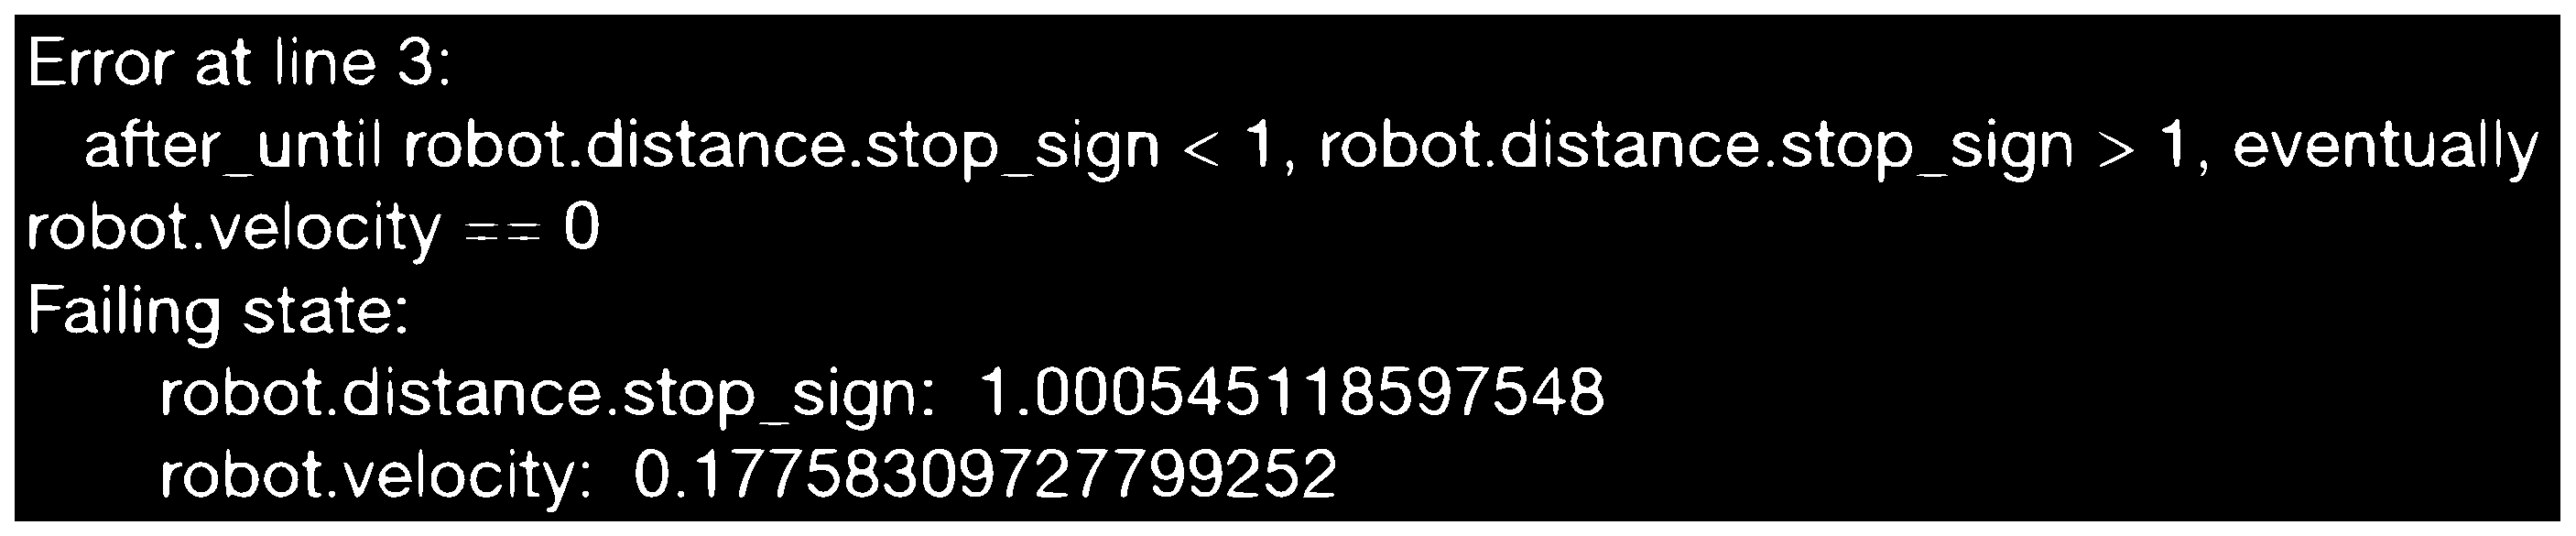
\includegraphics[width=\textwidth]{images/error.eps}
\caption{Example of the displayed error when the robot does not stop at the stop sign.} \label{fig:error}
\end{figure}

The flow of the process of monitoring a robotic system is described as follows:

\begin{enumerate}[label=(\roman*)]
    \item \textbf{Property formalization:} The developer describes in the DSL the properties of the robotic system one wants to monitor in a \texttt{.txt} file extension.
    \item \textbf{Compilation:} The specified properties are compiled, and a python file is generated capable of running as a ROS node.
    \item \textbf{Monitoring:} The node can be run whenever testing the system and will listen to pertinent topics and perform the computations needed to verify the specified properties.
\end{enumerate}


% ------------------------------------------------------------------------------
% Contributions
\section{Contributions}
\label{sec:contributions}

The expected contributions of this thesis are below enumerated.

\begin{enumerate}
    \item Definition of a domain-specific language to specify robotic systems' properties.
    \item Implementation of a compiler for the language that can generate software capable of monitoring relevant components while in a simulation.
    \item Evaluation of the expressive capabilities of the solution.
\end{enumerate}


% ------------------------------------------------------------------------------
% Structure of the document
\section{Structure of the document}
\label{sec:structure}

The document is organized as follows:

\begin{itemize}
    \item \autoref{chap:background} - Background \& Related Work:
    \item \autoref{chap:language} - Specification Language for Robotics Properties
    \item \autoref{chap:monitoring} - Monitoring
    \item \autoref{chap:evaluation} - Evaluation 
    \item \autoref{chap:futurework} - Future Work
    \item \autoref{chap:conclusion} - Conclusion
\end{itemize}

% !TeX root = ../main.tex
\chapter{Background \& Related Work}
\label{chap:background}

*Write structure after writing everything*

\section{Software}

*structure*

% ------------------------------------------------------------------------------
% ROS
\subsection{Robot Operating System}
\label{sec:ros}

The Robot Operating System (ROS)~\cite{quigley2009ros} is an open-source framework with a vast collection of libraries, interfaces, and tools that were designed to help build robot software. ROS provides an abstraction between hardware and software that helps developers easily connect the different robot components through messages sent through communication channels (\textit{topics}).

ROS has a modular architecture along with other advantages that were built with the purpose of cross-collaboration and easy development. For all these reasons ROS is used by hundreds of companies and research labs.

% ------------------------------------------------------------------------------
% Gazebo
\subsection{Gazebo}
\label{sec:gazebo}

Robotic systems simulation is an essential tool for testing robots' behavior, for this reason, Gazebo~\cite{koenig2004design} started with the idea of a high-fidelity simulator to simulate robots in any type of environment under mixed conditions.

Gazebo is an open-source 3D simulator that supports tools like sensors simulation, mesh management, and actuators control under different physics engines, among others, which makes it a simulator that can be used by very distinct robotic systems.

% ------------------------------------------------------------------------------
% Linear Temporal Logic
\section{Linear Temporal Logic}
\label{sec:ltl}

Linear temporal logic (LTL) is a branch of logic responsible for representing and reasoning about modalities in reference to time. 

As an approach for program verification, a formal system of temporal logic was suggested for both sequential and parallel programs~\cite{pnueli1977temporal}. LTL can be used as a method of model-checking~\cite{dwyer1998property} using its patterns as a form of property specification. It includes patterns such as "always", "finally", "until", "eventually", and others, which can be useful in the creation of invariants for program verification.

% ------------------------------------------------------------------------------
% Property Specification
\section{Robot Testing}
\label{sec:robottesting}

\subsection{Invariants}
%https://clairelegoues.com/papers/zizyte21dsn.pdf
%~\cite{zizyte2021importance}

\subsection{Runtime Monitoring}
%https://rose-workshops.github.io/files/rose2022/papers/RoSE22_paper_4.pdf
%~\cite{stadler2022towards}

\subsection{Similar work}
%ROSMonitoring~\cite{ferrando2020rosmonitoring}
%ROSRV~\cite{huang2014rosrv}

% !TeX root = ../main.tex
% %%%%%%%%%%%%%%%%%%%%%%%%%%%%%%%%%%%%%%%%%%%%%%%%%%%%%%%%%%%%%%%%%%%%%%%%%%%%%%
% Proposed Approach
\chapter{Proposed Approach}
\label{chap:approach}


The proposed approach consists initially in creating a domain-specific language.
The language will serve as a way to describe the properties of a robot.
For instance, if our robot is an autonomous car navigating on the road, 
one property could be that the robot stops at stop signs.
To describe robot properties, we also need the description of the testing scenario.
In the above example, the "road" and "stop sign" should be defined in the language as part of the 
testing scenario, without it there would be no way to describe the above property effectively.
To describe the scenario itself we can use GzScenic~\cite{GzScenic} in order to take 
advantage of the arbitrary creation of multiple scenario possibilities.
This language will then be composed of a new domain-specific language in association 
with the already established GzScenic language.

\par

Next in the approach, there is a need to build a compiler for the proposed language.
The compiler should be able to interpret a property in the language and be able to
identify the components of the robot necessary to monitor the said property.
The monitorization could take place either during runtime or after using log files.
Taking the above example into account, our compiler should have the information of which 
component of the robot is responsible for the car position as well as the position of the 
stop sign, it can then monitor the component and check if the property has been broken.

\par

The language should be of high level in the sense that it should be intuitive to the writer.
With this approach, the person doing the robot testing shouldn't need so much in-depth 
knowledge about the robot to perform a test. This is because of the writing simplicity of 
the language and the removal of the manual labor side of personally monitoring the robot.

\par

The final scheme of the tool proposed is represented in the below diagram.

\begin{figure}[h!]
    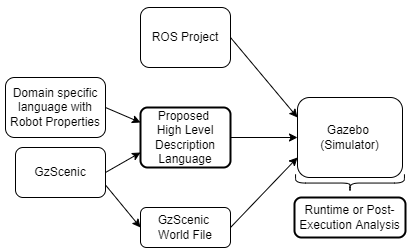
\includegraphics{images/intro_diag.png}
    \caption{Tool for monitoring robot properties.}
    \label{fig:intro_objectives}
\end{figure}

% Appendixes
\appendix
% !TeX root = ../main.tex
% %%%%%%%%%%%%%%%%%%%%%%%%%%%%%%%%%%%%%%%%%%%%%%%%%%%%%%%%%%%%%%%%%%%%%%%%%%%%%%
% Appendixes
\chapter*{Appendix A}
\label{app:appendix-A}

\section{Displayed Error messages}

\begin{figure}
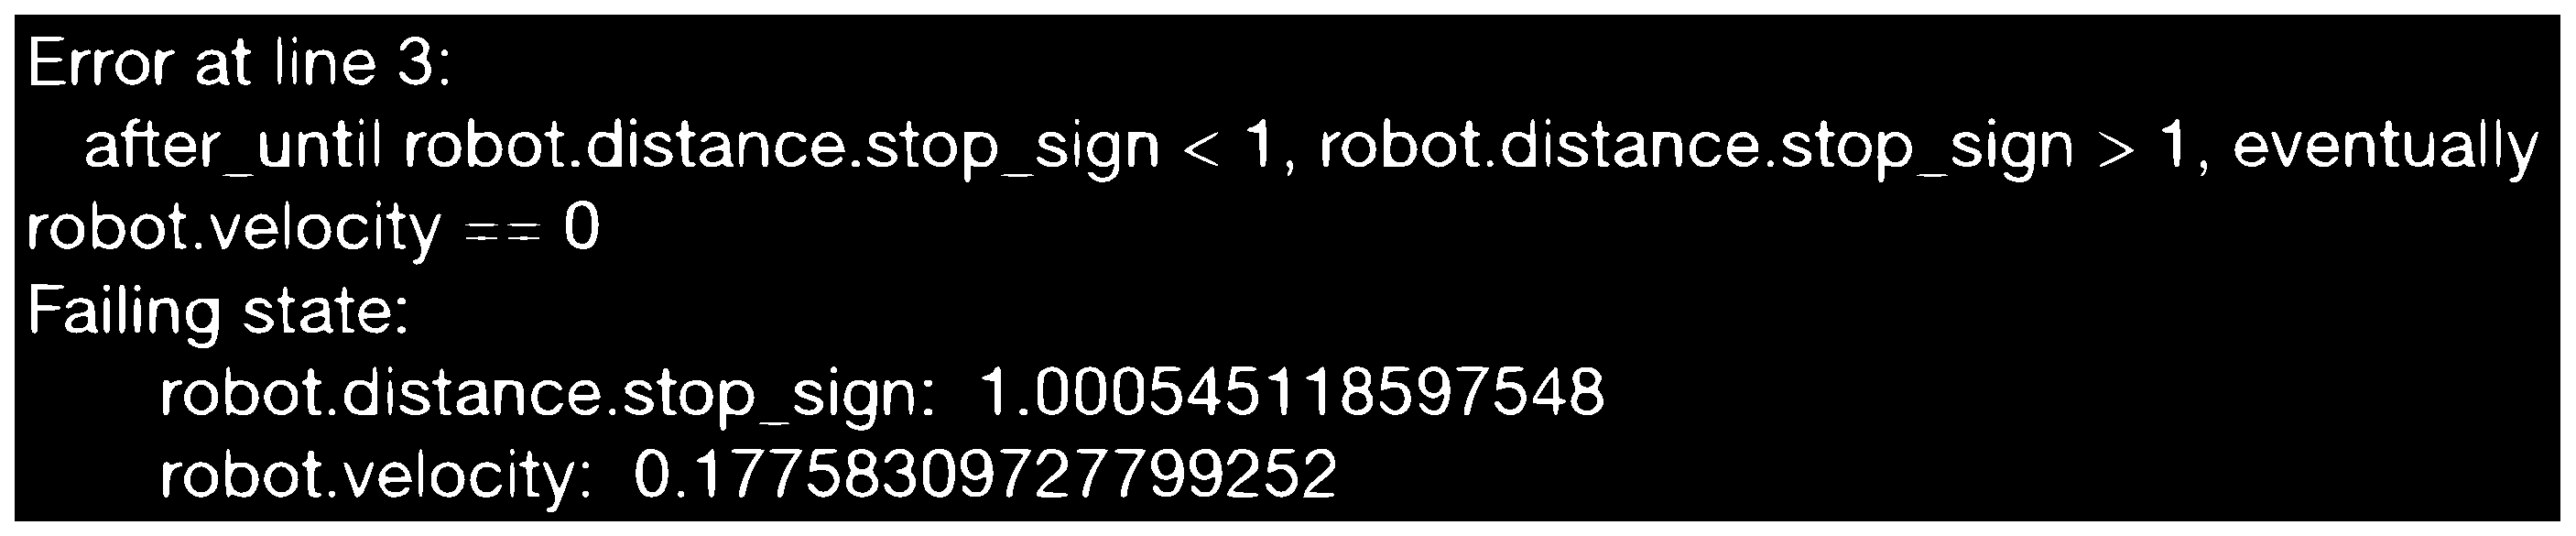
\includegraphics[width=\textwidth]{images/error.eps}
\caption{Example of the displayed error when the robot does not stop at the stop sign.}
\end{figure}

\begin{figure}[h]
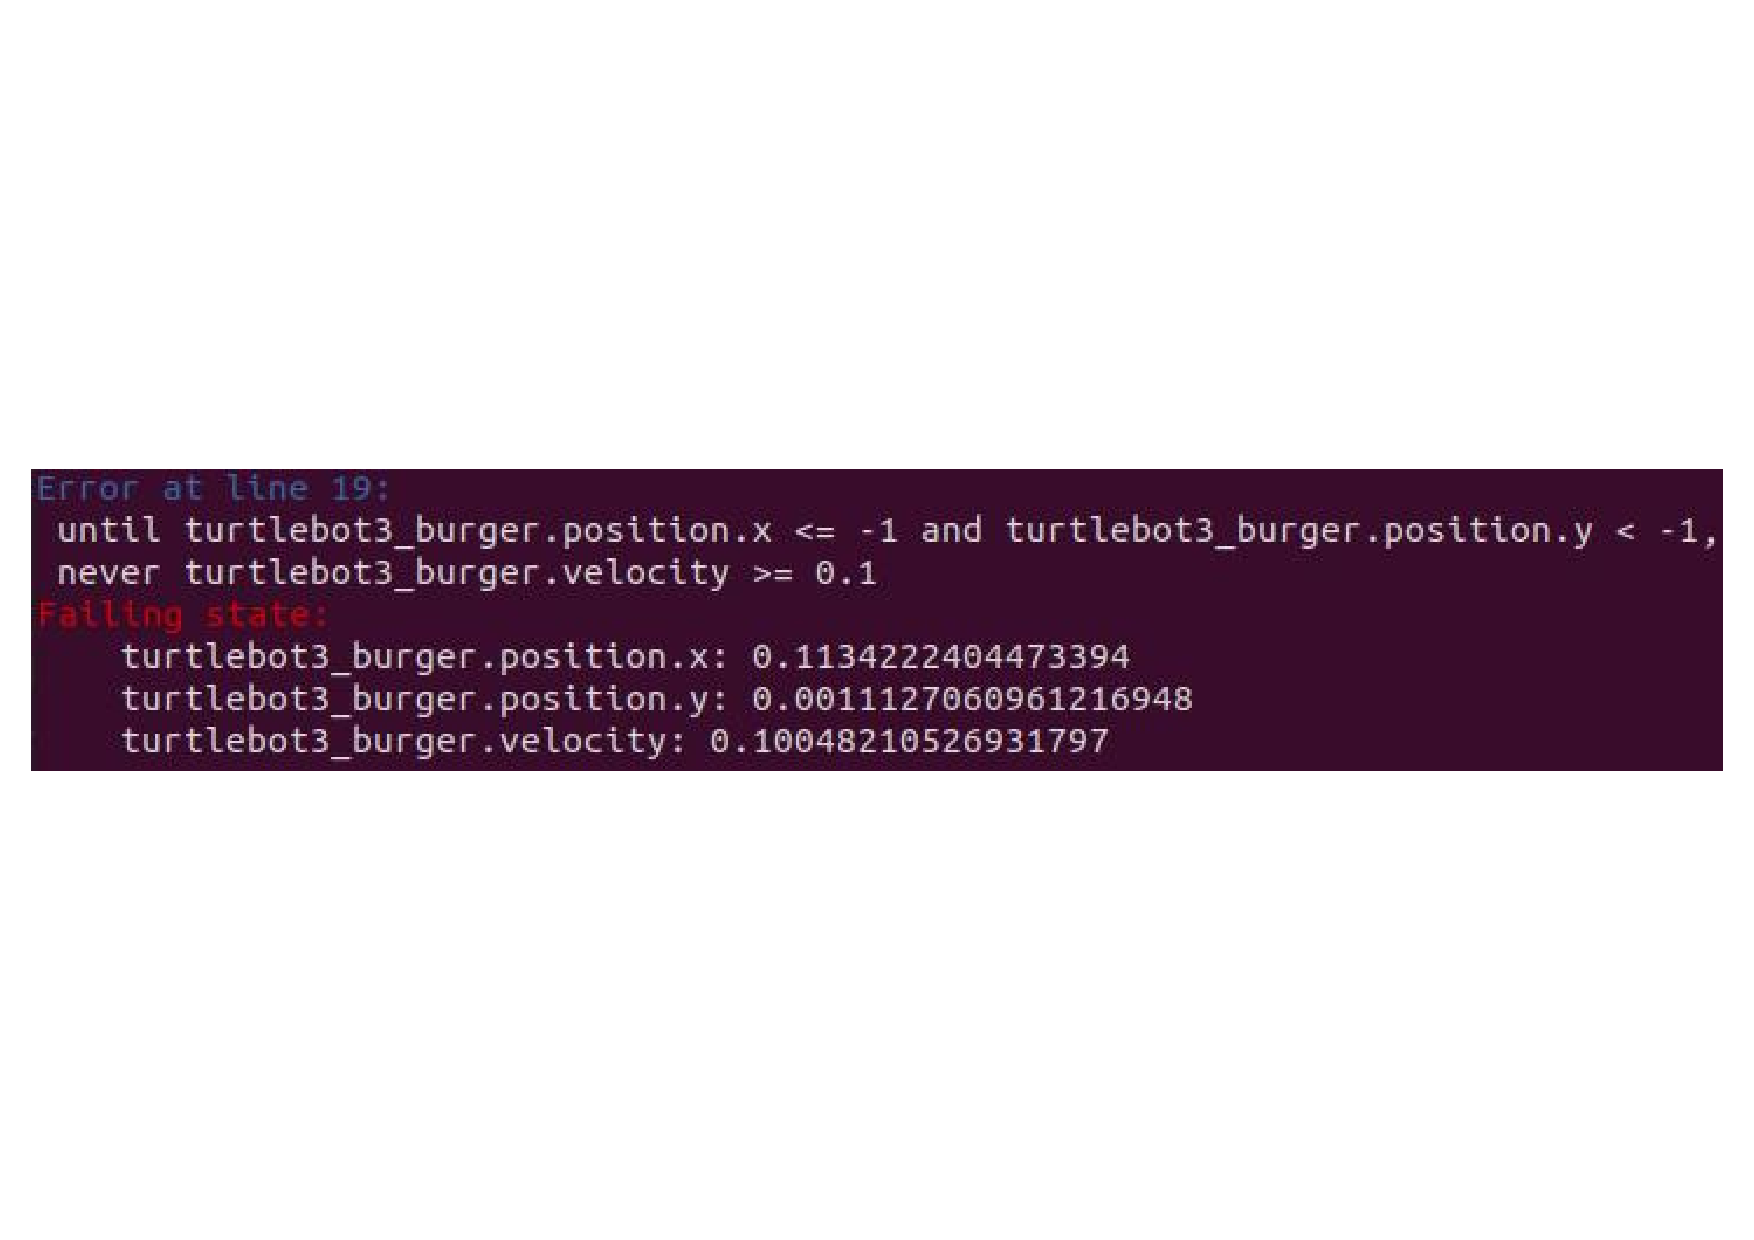
\includegraphics[width=\textwidth]{images/error_message.pdf}
\caption{Example of an error message.}
\end{figure}

\begin{figure}
\begin{center}
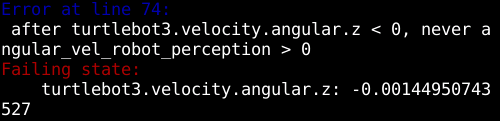
\includegraphics[width=8cm,height=2cm,keepaspectratio,]{images/erreval1.png}
\caption{Calculation Error Inverts Turning Direction bug error message.}
\end{center}
\end{figure}

\begin{figure}
\begin{center}
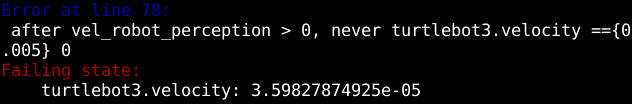
\includegraphics[width=10cm,height=3cm,keepaspectratio,]{images/erreval2.png}
\caption{Robot Getting Stuck When Auto-docking bug error message.}
\end{center}
\end{figure}

\begin{figure}
\begin{center}
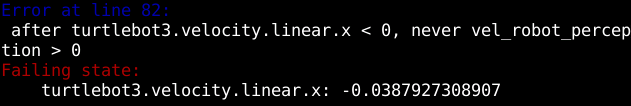
\includegraphics[width=10cm,height=3cm,keepaspectratio,]{images/erreval3.png}
\caption{Unexpected Movement Due to Wrong Calculation bug error message.}
\end{center}
\end{figure}


\chapter*{Appendix B}
\label{app:appendix-B}

\section{Evaluation Flow Diagrams}

\begin{figure}
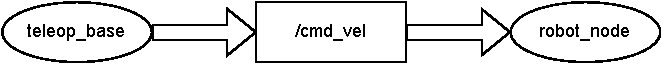
\includegraphics[width=\textwidth]{images/normal_flow.pdf}
\caption{The normal runtime flow of the system.}
\end{figure}
       
\begin{figure}
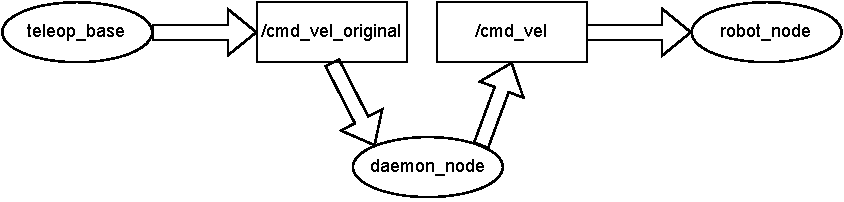
\includegraphics[width=\textwidth]{images/demon_flow.pdf}
\caption{The flow of the system when the adding the demon node.}
\end{figure}


% Bibliography
\bibliography{references}
\addcontentsline{toc}{chapter}{References}

\end{document}